%=========================================================================
\documentclass[11pt,twoside,a4paper]{article}
\usepackage[dutch]{babel}
\usepackage{a4wide,times}
\usepackage{pdfpages}
\usepackage{graphicx}
\usepackage{float}
\usepackage{rotating}
\usepackage{listings}
\usepackage{hyperref}
\usepackage{enumitem}
\newenvironment{myitemize}
{ \begin{itemize}[topsep=1ex]
    \setlength{\itemsep}{5pt}
    \setlength{\parskip}{5pt}
    \setlength{\parsep}{5pt}     }
{ \end{itemize}                  }
\title{Module-opdracht: Arithmatic Logic Unit (ALU)}
\author{
Gemaakt door leden van projectgroep A1\\
Joran Out, 4331958\\
Alex Oudsen, 4325494\\
\\
In opdracht van \\
Roy Blokker, 4148894\\
Elke Salzmann, 4311450\\
}
\date{26 November 2014\\Versie 1.0}
\begin{document}
\maketitle
\thispagestyle{empty}
\vspace{30 mm}
\begin{center}
\Large \bf 
Samenvatting
\end{center}
Dit document beschrijft het ontwerp van een Arithmetic Logic Unit (ALU) voor de zogenaamde moduleopdracht bij het EPO-3 project van de opleiding Electrical Engineering aan de TU Delft. Een ALU is een module die op een chip wordt ingezet voor het uitvoeren van rekenkundige en logische bewerkingen. De ALU in dit verslag is ontworpen op basis van een opdracht, welke specificeert dat de ALU in staat dient te zijn tot optellen, aftrekken, naar links- en rechts verschuiven \& de logische operaties NOT, AND, OR en XOR. Het ontwerpen van de ALU gebeurt in het IC-ontwerpprogramma \emph{GoWithTheFlow}, waarbinnen nog vele andere programma's worden gebruikt; bijvoorbeeld voor het simuleren van VHDL en het genereren van een layout voor de ontworpen schakeling op een Sea-of-gates chip. De ontworpen ALU en een bijpassende testbench zullen worden beschreven in VHDL, waarbij gebruik gemaakt wordt van diagrammen om de omzetting naar VHDL te vereenvoudigen. Vervolgens wordt het ontwerp op verschillende logische niveau's gesimuleerd in \emph{GoWithTheFlow}, van de ruwe VHDL-code tot op transistorniveau. De benodigde tussenstappen als het genereren van een layout  kunnen hierbij geautomatiseerd worden uitgevoerd binnen de ontwerpomgeving. Op deze manier kan worden gecontroleerd of het ontwerp het gespecificeerde gedrag vertoont. Ten slotte worden de verkregen resultaten van de verscheidene simulaties vergeleken met de aangeleverde specificaties, zodat aan de opdrachtgevers kan worden getoond dat de ontworpen module hieraan voldoet.
\clearpage

\tableofcontents
\clearpage

\section{Inleiding}
In dit verslag wordt het ontwerpproces van een Arithmetic Logic Unit (ALU) behandeld. Dit ontwerp is uitgevoerd in het kader van de zogenaamde moduleopdracht behorend bij het EPO-3 project van de opleiding Electrical Engineering aan de TU Delft. Deze moduleopdracht houdt in dat een tweetal leden van de projectgroep opdracht geeft tot het ontwerp van een zogenaamde 'module' voor op een Sea-of-gates chip. Hierbij is een module een schakeling op een chip met een bepaalde functie, welke over het algemeen vaak gebruikt wordt. Twee andere groepsleden dienen deze opdracht uit te voeren volgens de specificaties van de opdrachtgevers. Deze specificaties bevatten in ieder geval informatie over de functionaliteit, in- en uitgangssignalen en testbaarheid van de te ontwerpen module. Ook eventuele randvoorwaarden dienen in de specificaties te zijn opgenomen. Het op te leveren resultaat van de opdracht bestaat uit de ontworpen ALU in behavioural VHDL, een geschikte testbench in VHDL en dit verslag, dat onder andere ook de simulatieresultaten van het ontwerp op de verschillende logische niveau's dient te bevatten. De offici\"ele beschrijving van de Module opdracht is ten slotte te vinden in hoofdstuk 14 van de handleiding behorend bij het EPO-3 project \cite{Handleiding}, welke ook online via blackboard beschikbaar gesteld is \cite{Handleiding_bb}.

\section{Specificaties}
Zoals in de inleiding al is aangegeven, zijn de specificaties van de te ontwerpen ALU opgesteld door een ander tweetal leden van de projectgroep. Deze specificaties zijn in overleg met de opdrachtgevers en de groepsbegeleiders van het EPO-3 project zo aangepast dat duidelijk is wat er precies van de ontwerpen ALU verwacht wordt. Bovendien is in de complexiteit van de specificaties rekening gehouden met een beschikbare tijd van drie dagdelen \`a vier uur voor de uitvoering van de opdracht. Hierop volgend zijn de uiteindelijk vastgestelde specificaties letterlijk in dit verslag overgenomen:
\includepdf{Specs_ALU_3_0.pdf}

\section{Ontwerp}
De eerste stap in het ontwerpproces van de ALU begint met de interpretatie van de vastgestelde specificaties. Hoewel over de meeste punten in deze specificaties geen onduidelijkheid bestaat, wordt hier voor de duidelijkheid nog wel een overzicht van de specificaties gegeven zoals deze zijn ge\"interpreteerd tijdens het ontwerpen van de module:
\begin{myitemize}
\item De ALU dient te reageren op de rising edge van de ingang klok (clk) waarop deze gaat werken. Dit houdt in dat de uitgangssignalen alleen mogen veranderen bij een opgaande klokflank.
\item De ingangen A en B zijn 4-bits vectoren in 2's complement representatie waarop de verschillende bewerkingen worden gedaan die de ALU uit moet gaan kunnen voeren. Afhankelijk van de uit te voeren operatie wordt of alleen signaal A of worden beide signalen gebruikt.
\item Het resultaat van de bewerkingen wordt weggezet in een register met de huidige uitgangswaarden van de ALU, welke het resultaat (4 bits) en de carry (1 bit) zal bevatten. Dit betekent praktisch gezien dat de uitgang van de ALU wordt behouden zolang deze niet wordt overschreven door het reslutaat van een volgende operatie. Wat er precies aan welke uitgang terecht komt is afhankelijk van de uit te voeren operatie.
\item Het 3-bits ingangssignaal F dient ten slotte te worden ge\"inplementeerd als een selectiesignaal, waarmee kan worden aangegeven welke van de volgende acht opgegeven functies de ALU moet gaan uitvoeren:
\begin{enumerate}
\item A + B (geeft een 5-bits resultaat, met de MSB in de carry)
\item A - B (geeft een 5-bits resultaat, met de MSB in de carry)
\item Left-shift A (MSB in de carry \& LSB wordt '0')
\item Right-shift A (carry en MSB '0' \& LSB gaat verloren)
\item A AND B (carry '0')
\item A XOR B (carry '0')
\item A OR B (carry '0')
\item NOT A (carry '0')
\end{enumerate}
Welke waarde van F wordt toegekend aan welke van deze functies is overgelaten aan de ontwerpers. Er is uiteindelijk gekozen voor de uitwerking van tabel \ref{representatie}:\\
\begin{table}[H]
\begin{center}
\caption{Overzicht gekozen representatie van de functies van de ALU in F}
\label{representatie}
\begin{tabular}{|l | c |}
\hline
Functie van de ALU & Binaire waarde van F\\
\hline
NOT A & "000"\\
A OR B & "001"\\
A AND B & "010"\\
A XOR B & "011"\\
A + B & "100"\\
A - B & "101"\\
Left-shift A & "110"\\
Right-shift A & "111"\\
\hline
\end{tabular}
\end{center}
\end{table}
\end{myitemize}

\subsection{Blokrepresentatie van de ALU}
Een eerste stap in de omzetting van specificaties tot VHDL-ontwerp van de ALU, is het opstellen van een black-box-model van de ALU zoals in figuur \ref{Blokrepresentatie}. In dit figuur is de ALU weergegeven als een blok, dat verschillende logische onderdelen (logic units) bevat. Hiermee wordt aangegeven dat het blok ALU een module is die logica implementeert. Verder worden in dit simpele diagram alle ingangen samengenomen tot een blok signal aan de ingang van de ALU en alle uitgangen tot een blok output aan de uitgang van de blokrepresentatie van de ALU.
\begin{figure}[H]
\begin{center}
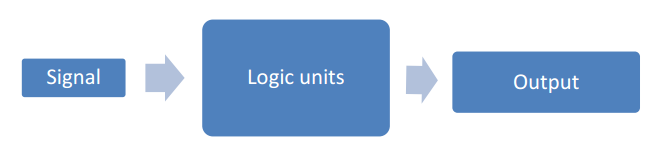
\includegraphics[keepaspectratio=true,scale=0.85]{Blokrepresentatie.png}
\caption{Blokrepresentatie van de ALU}
\label{Blokrepresentatie}
\end{center}
\end{figure}

\subsection{Opdeling in deelschakelingen}
Met behulp van figuur \ref{Blokrepresentatie} is het echter nog niet mogelijk om de ALU direct in VHDL te implementeren. Daarom worden extra details aan dit diagram toegevoegd, door verschillende deelschakelingen en -signalen te introduceren. Dit geeft een nieuw blokdiagram, welke wordt weergegeven in figuur \ref{Deelblokken}. In dit diagram zijn de verschillende functies van de ALU nu te onderscheiden. Ook zijn de uitgangssignalen nu gesplitst. Dit diagram is echter ook nog niet volledig genoeg voor een VHDL-beschrijving.
\begin{figure}[H]
\begin{center}
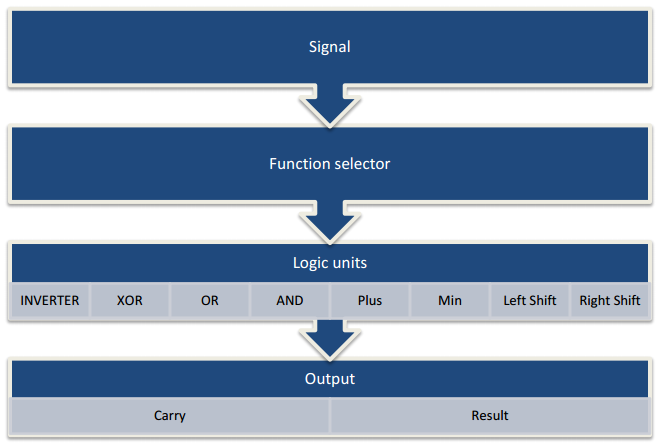
\includegraphics[keepaspectratio=true,scale=0.9]{Deelblokken.png}
\caption{Opdeling van de ALU in verschillende deelblokken}
\label{Deelblokken}
\end{center}
\end{figure}

\subsection{Omzetting van diagram tot VHDL}
De module-opdracht vraagt om een resultaat in behavioural VHDL. Het uiteindelijke doel is dan ook om de ALU-module, zoals deze in de specificaties wordt beschreven, om te zetten in een behavioural VHDL beschrijving. Figuren \ref{Blokrepresentatie} en \ref{Deelblokken} bleken hiervoor niet gedetailleerd genoeg. Daarom wordt het blokdiagram nog verder uitgebreid, wat figuur \ref{Overzicht} oplevert.
\begin{figure}[H]
\begin{center}
\includegraphics[keepaspectratio=true,scale=1.1]{Blokken_en_signalen.png}
\caption{Overzichtsweergave van de ALU in blokken met bijbehorende signalen}
\label{Overzicht}
\end{center}
\end{figure}
\noindent Nu is duidelijk te zien hoe de ALU ge\"implementeerd moet gaan worden in VHDL. Alle gespecificeerde in- en uitgangssignalen zijn nu aan te wijzen. Bovendien is aangegeven welk signaal waar naar toe gaat. Ook is duidelijk te zien dat de functieselectie met behulp van het 3-bits signaal F het gemakkelijkste gerealiseerd kan worden met behulp van een case-statement. Ten slotte wordt getoond te zien hoe de registers aan de uitgang worden ge\"implementeerd. De implementatie van de arithmetische en logische bewerkingen van de ingangssignalen spreekt voor zich. De resulterende behavioural VHDL beschrijving van de ALU-module is terug te vinden in de appendix in sectie \ref{ALU-VHDL}. In deze beschrijving is voor de in- en uitgangssignalen de naamgeving van de figuur in de specificaties aangehouden, op het uitgangssignaal carry na, die wordt aangegeven met een c in plaats van een d.\\
Voor het testen van de geschreven VHDL wordt gebruik gemaakt van een testbench. Deze is ook geschreven in VHDL en terug te vinden in de appendix in sectie \ref{Testbench}.

\newpage
\section{Resultaten}
Met de beschrijving van de ALU en bijbehorende testbench in behavioural VHDL is het op te leveren product in principe af. Voordat deze files kunnen worden ingeleverd, moet echter wel eerst worden gecontroleerd of deze wel voldoen aan alle specificaties van de opdrachtgevers. Blijkt dit niet het geval, dan dient de VHDL beschrijving van de ALU zo te worden aangepast, dat dit wel het geval wordt. Het testen van de behavioural VHDL beschrijving van de ALU gebeurt in eerste instantie met behulp van de geschreven testbench in de VHDL simulator van \emph{Modelsim}. Het resultaat van deze simulatie is weergegeven in figuur \ref{Modelsim} in de appendix in sectie \ref{Testbench} en is veelbelovend: de ALU functioneert zoals verwacht en er lijkt aan alle specificaties van de opdrachtgevers te worden voldaan.

\subsection{Synthetiseren}
Een geslaagde simulatie op een hoog beschrijvend niveau als VHDL is echter nog geen bewijs dat de ontworpen ALU ook zal gaan werken op een Sea-of-gates chip. Daarom wordt binnen de omgeving van \emph{GoWithTheFlow} een logische synthese uitgevoerd op de VHDL beschrijving van de ALU, wat ervoor zorgt dat deze gedragsbeschrijving wordt omgezet in een netwerkbeschrijving bestaande uit cellen uit de Sea-of-Gates celbibliotheek. Ook deze beschrijving is in VHDL en kan dus worden gesimuleerd met behulp van \emph{Modelsim}. Het resultaat van deze simulatie is te vinden in figuur \ref{Synthesised} in de appendix in sectie \ref{Testbench} en is vrijwel identiek aan die van de simulatie van de VHDL behavioural beschrijving in figuur \ref{Modelsim} in dezelfde sectie. Het enige verschil is dat de uitgangssignalen nu onderhevig zijn aan enige vertraging. Deze vertraging is echter kort genoeg, zodat de ALU in staat blijft zijn operaties binnen \'e\'en klokperiode kan voltooien.

\subsection{Layout}
De gesynthetiseerde VHDL beschrijving van de ALU bevat echter nog geen informatie over de plaatsing van de Sea-of-gates cellen op een chip. Ook met de bedrading van deze chip is dus nog geen rekening gehouden. Daarom wordt binnen \emph{GoWithTheFlow} vanuit de gesynthetiseerde VHDL een layout gegenereerd met behulp van \emph{row placer} voor het plaatsen van de cellen en \emph{trout} in \emph{seadali} voor het automatisch genereren van de bedrading. Alternatief gezien had binnen \emph{seadali} ook het plaatsen en bedraden in \'e\'en keer gedaan kunnen worden met behulp van place \& route, welke \emph{Madonna} aanroept voor het plaatsen en \emph{trout} voor de bedrading. Het probleem is echter dat \emph{Madonna} de cellen zo compact mogelijk probeert te plaatsen, waardoor het voor komt dat \emph{trout} niet genoeg ruimte meer heeft voor het bedraden van alle cellen. Daarom is gebruik gemaakt van \emph{row placer}, zodat het aantal rijen cellen en de onderlinge afstand tussen de cellen handmatig vergroot kan worden. Dit zorgt er voor dat \emph{trout} genoeg ruimte heeft voor het bedraden van alle cellen, maar dit gaat wel ten koste van de efficiëntie van de schakeling. Om de validiteit van de gegenereerde layout te controleren, kan binnen \emph{GoWithTheFlow} een VHDL beschrijving van de layout worden ge\"extraheerd. Deze VHDL beschrijving kan vervolgens weer met behulp van \emph{Modelsim} worden gesimuleerd. Het resultaat van deze simulatie is weergegeven in figuur \ref{Extracted} in de appendix in sectie \ref{Testbench}. Deze simulatie geeft hetzelfde resultaat als de simulatie van de gesynthetiseerde VHDL in figuur \ref{Synthesised}. Dit betekent dat de gegenereerde layout overeenkomt met de VHDL netwerkbeschrijving van de ALU.

\newpage
\subsection{Switch-level simulatie}
Naast de zojuist beschreven controlewijze bestaat er nog een tweede manier om te controleren of de gegenereerde layout overeenkomt met de VHDL netwerkbeschrijving. Dit gebeurd door middel van een zogenaamde switch-level simulatie. Deze simulatie wordt uitgevoerd door de \emph{PSPICE} simulator en beschouwt de transistoren in het ontwerp als schakelaars. Deze andere aanpak is over het algemeen een nauwkeurigere manier van verificatie, omdat deze ervoor zorgt dat problemen als spikes of glitches naar voren kunnen komen die in een simulatie met \emph{Modelsim} onopgemerkt blijven. Het resultaat van de switch-level simulatie is weergegeven in figuur \ref{Switch-level} in de appendix in sectie \ref{Testbench}. Doordat deze simulatie is uitgevoerd door \emph{PSPICE} in plaats van \emph{Matlab}, is het niet zo eenvoudig om het resultaat van de switch-level simulatie te vergelijken met die van de VHDL netwerkbeschrijving. Binnen \emph{GoWithTheFlow} bestaat echter de optie om beide simulaties automatisch met elkaar te laten vergelijken. Hierbij worden vlak voor iedere opgaande klokflank de uitgangssignalen van beide simulaties met elkaar vergeleken. De resultaten van deze vergelijking zijn weergegeven in figuur \ref{Vergelijking}. In de figuur is te zien dat deze vergelijking alleen een foutmelding geeft tijdens de eerste klokperiode. Tijdens de eerste klokperiode is de initialisatie van het systeem echter nog niet helemaal voltooid, waardoor de uitgangssignalen van het systeem nog niet eenduidig gedefiniëerd zijn. De uitgangssignalen van beide simulaties zijn op dit moment dus nog willekeurig, wat het logisch maakt dat ze niet met elkaar overeenkomen.
\begin{figure}[H]
\begin{center}
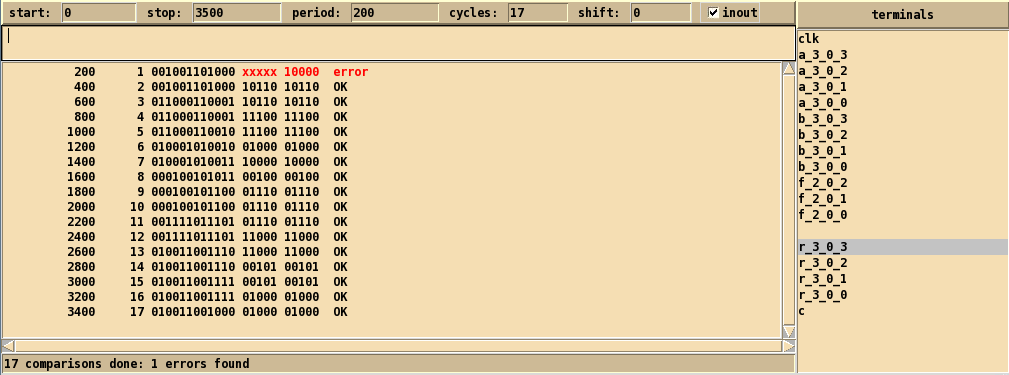
\includegraphics[keepaspectratio=true,scale=0.8]{Comparison.png}
\caption{Vergelijking resultaten behavioural VHDL- en Switch-level simulaties}
\label{Vergelijking}
\end{center}
\end{figure}

\newpage
\section{Conclusies}
Zoals gebleken uit de verschillende simulaties, kan de ontworpen ALU-module op basis van een 3-bits ingangssignaal \'e\'en van de acht vastgestelde operaties uitvoeren op \'e\'en of twee 4-bits ingangssignalen, welke zijn gecodeerd in 2's complement. Bijbehorende uitganssignalen worden volgens specificatie bewaard totdat er nieuwe uitganssignalen beschikbaar zijn. De ALU voldoet bovendien aan de eisen om de operaties te starten op de opgaande klokflank en te voltooien binnen \'e\'en klokperiode. Ten slotte bestaan de uitganssignalen van de ALU, zoals gespecificeerd, uit een 4-bits signaal resultaat en een carry-signaal van 1 bit.\\
\\
Ondanks het feit dat de ALU voldoet aan de specificaties, zouden er voor een volgende opdracht nog verdere toepassingen of verbeteringen ge\"implementeerd kunnen worden. Zo zouden er bijvoorbeeld meer functies ge\"implementeerd kunnen worden. Daarnaast zou er een functie toegevoegd kunnen worden waarbij de ALU zijn laatste resultaat kan gebruiken als input. Ten slotte zou ook het toevoegen van een (synchrone) reset, een signaal dat nu niet in de specificaties is opgenomen, een mogelijkheid bieden om de registers aan de uitgang leeg te maken.


\begin{thebibliography}{9}
\bibitem{Handleiding}
Bakker, A. et al., 
\emph{Handleiding practicum Ge\"integreerde Schakelingen en project Ontwerp een Chip},
De Module opdracht,
TU Delft, 
September 2014,
pp. 68.
\bibitem{Handleiding_bb}
Handleiding GS en EPO-3, 
\url{https://blackboard.tudelft.nl/bbcswebdav/pid-2389635-dt-content-rid-7944763_2/courses/34308-141502/handleiding_GS_EPO3.pdf}, 
geraadpleegd op 23 nov. 2014.
\end{thebibliography}

\newpage
\section{Appendix A: ALU in VHDL
\label{ALU-VHDL}}
\lstinputlisting{alu.vhdl}
\hrule
\lstinputlisting{behaviour.vhdl}
\newpage
\section{Appendix B: Testbench en simulatieresultaten}
\label{Testbench}
\lstinputlisting{alu_tb.vhdl}
\hrule
\lstinputlisting{alu_tb_behaviour.vhdl}

\begin{sidewaysfigure}
\begin{center}
\includegraphics[keepaspectratio=true,scale=1.0]{Modelsim_simulatie_stacked.png}
\caption{Simulatieresultaat behavioural VHDL beschrijving}
\label{Modelsim}
\end{center}
\end{sidewaysfigure}
\begin{sidewaysfigure}
\begin{center}
\includegraphics[keepaspectratio=true,scale=1.0]{Synthesised_simulatie_stacked.png}
\caption{Simulatieresultaat gesynthetiseerde VHDL beschrijving}
\label{Synthesised}
\end{center}
\end{sidewaysfigure}
\begin{sidewaysfigure}
\begin{center}
\includegraphics[keepaspectratio=true,scale=1.0]{Extracted_simulatie_stacked.png}
\caption{Simulatieresultaat geëxtraheerde VHDL beschrijving}
\label{Extracted}
\end{center}
\end{sidewaysfigure}
\begin{sidewaysfigure}
\begin{center}
\includegraphics[keepaspectratio=true,scale=0.58]{Switch-level_simulatie.png}
\caption{Switch-level simulatieresultaat}
\label{Switch-level}
\end{center}
\end{sidewaysfigure}
\end{document}